\documentclass[conference, 12pt, onecolumn]{IEEEtran}
\usepackage{cite}
\usepackage{graphicx}
\usepackage{textcomp}
\usepackage{xcolor}

\date{}

\begin{document}
\title{Maskit: COVID-19 Resiliency through Computer Vision and Robotics}
\author{ \IEEEauthorblockN{Allen Mao}
\IEEEauthorblockA{University of California, Berkeley \\ Berkeley, California \\ \texttt{allenmao@berkeley.edu}}
\and
\IEEEauthorblockN{Hans Gundlach}
\IEEEauthorblockA{University of California, Berkeley \\ Berkeley, California \\ \texttt{11235hans@berkeley.edu}}
}

\maketitle
\tableofcontents
\newpage

\section{Introduction}
The COVID-19 pandemic has led to, at the time of this writing, almost half a million deaths, the worst global recession since the Great Depression, and school closures that have affected nearly all of the world's student population. Although reopening efforts have been underway in many parts of the world, their results have been mixed and it is often instead in citizens' own hands to protect themselves from this virus through means such as social distancing, frequent handwashing, and mask wearing. Although the United States Centers for Disease Control and Prevention (CDC) has issued recommendations for citizens to wear masks to reduce exposure to the virus, the choice to wear a mask has unfortunately evolved to become a political question too\cite{brandon_2020, vigdor_2020}. Apart from CDC and World Health Organization (WHO) guidelines to wear facial coverings, i.e. masks, in this article we will not discuss the merits of face coverings; this knowledge is assumed. Instead, we propose, describe, and demonstrate \textit{Maskit}, a computer vision and robotics system that keeps business owners and other ordinary citizens safe by blocking people who fail to wear a mask while letting people who do through entrances.
\subsection{Code Source}
% insert github link here
\section{Purpose \& Motivation}
% insert personal bios and anecdotes here:
We are both undergraduate students at the University of California, Berkeley. Allen is a Computer Science major who is primarily interested in Natural Language Processing
% Allen is CS major at UCB and Hans is math + physics. They met at International House. Little did they know that semester would be so abruptly cut off by a pandemic. (Detail brutal dining conditions at I house.) Shock and horror at news coming in about so much death.
% Video of Costco customer refusing to wear a mask. Customers like this are selfish and endanger other people's safety. Even worse, store employees have to personally go escort the person out--who knows how many people this person could infect in that time period? Better, have a computer analyze people automatically: computers can't get infected with COVID and now store employees aren't putting their lives at risk thanks to selfish bass turds.
% This inspired us to think about creating such a system. 
\subsection{Previous Work on Mask Identification with Computer Vision}
In the past several months, several organizations, for example Didi Chuxing\footnote{https://github.com/didi/maskdetection} and AI Zoo Tech\footnote{https://github.com/AIZOOTech/FaceMaskDetection} have released open-source pre-trained neural network models on multiple platforms (Keras, Tensorflow, and Caffe) that classify faces within a photo or video as mask-wearing or not. Both models perform spectacularly as the Didi model was trained on a dataset of over 200,000 faces while the AIZOO model consists of 24 convolutional layers trained on approximately 8000 images from WIDER Face and MAFA datasets. Accordingly, the Didi model achieves at least 98\% accuracy and the AIZoo model has a 0.896 ROC AUC (\textit{receiver operating characteristic area under the curve} for face detection and 0.919 ROC AUC for face mask detection, as seen in their curve below.
\begin{center}
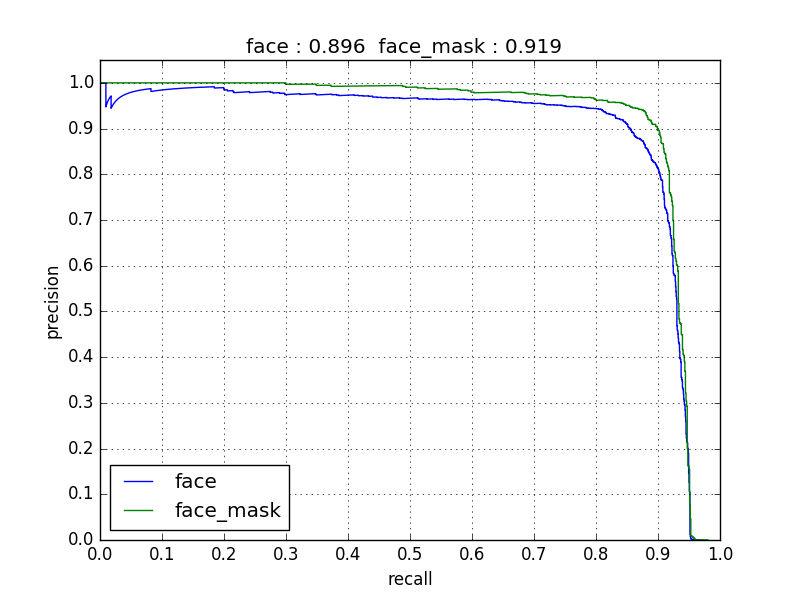
\includegraphics[scale=.5]{pr_curve}
\end{center}


% Computer vision for mask detection
% Computer vision for identifying mask type
\subsection{What is \textit{Maskit}.}
Maskit 
%Google search revealed trained Tensorflow models that recognized human faces. Hans had experience with TF. Allen had experience working with R Pis and servo controls blabla. Combined forces to bring this product together.
%They've come up with prototype that consists of a Rpi and a server. The Rpi is connected to Camera module and servo. It takes pictures at intervals and sends to server as POST request. Server processes pictures with TF model and identifies human faces as masked or unmasked. Then, sends this as response to POST request. If all people identified are wearing a mask, then the raspberry pi activates a welcome flag. Else, people denied entry.
%In model, we have welcome flag, but this can be generalized to any motor, e.g. sliding doors at supermarkets, bolts for regular doors, etc.


\section{Step by Step Usage Instructions}
\subsection{Setting up the server}

\subsection{Running it on R Pi}
The raspberry pi is 

\section{Difficulties and Challenges}
We faced many challenges during the completion of the project. We tried to do all the image processing on the raspberry pi however the pi, unfortunately, did not have either the necessary speed or space to handle the complicated image processing in OpenCV and Tensorflow. Therefore, we had to design an HTTP server using python to send the image to a Linux computer where the image is processed. Finding the right model for mask detection was also difficult. We tried several different frameworks before finding an efficient Tensorflow mask detection model from AIZOO. Remote work also proved difficult especially for a hardware project where only one of us could see the immediate results.
\section{Market Evaluation}
MaskIt has several market application. MaskIt could be used as an artificial bouncing mechanism to ensure that people use masks in public places. Large scale mask detection could also be useful in epidemiological and policy research. 
\section{Suggested Improvements}
MaskIt needs to be fully evaluated in larger public situations. If it is going to be useful in public places 
\section{Conclusion}
In conclusion, MaskIT has significant potential in research and commercial settings during the COVID pandemic. Given the lack of curret data on mask usage in practice and the importance of mask in the current public health it is important to create automated systems to tack account of mask usage. Some building may need automated gate systems to scan mask usage while universities will need to monitor the percentage of mask compliance on campuses. Systems like MaskIT will be of increasing public importance in the coming months. 

\bibliographystyle{ieeetr}
\bibliography{citations}


\end{document}
